\chapter{Gestion d'utilisateurs : UserBundle}

Les fonctionnalités liées aux utilisateurs sont situés dans le UserBundle. Ce bundle contient toutes les fonctionnalités permettant aux utilisateurs d'effectuer les actions l'affectant lui même ou un autre utilisateur. On peut subdiviser ce bundle en trois: une partie commune, la partie concernant les étudiants et une partie concernant les administrateurs.

\section{Gestion d'utilisateurs générale}

\subsection{Login}

Lorsque un utilisateur à été ajouté à la base de donnée, il peut se connecter au site grâce à ses identifiants INSA qui sont vérifiés grâce au LDAP (cf figure \ref{log}).

\begin{figure}[H]
	\centering
	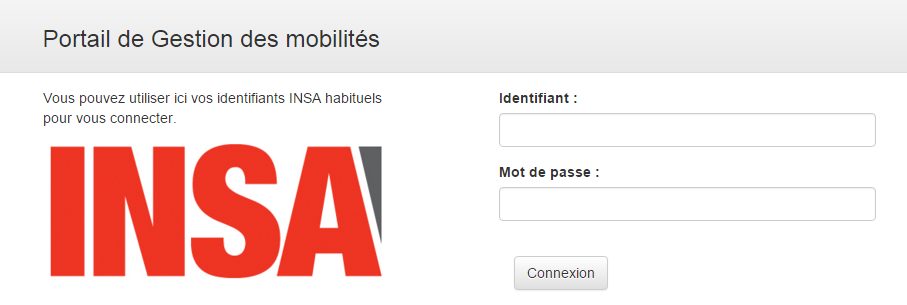
\includegraphics[scale=0.35]{images/log.png}
	\caption{Page de login}
	\label{log}
\end{figure}

\subsection{Résumé des vœux}

Les utilisateurs peuvent avoir accès par plusieurs moyens à un résumé des vœux. Sur la page d'accueil de chaque élève, le résumé de ses vœux. Sur la page d'accueil des administrateurs, le résumé de tout les vœux des élèves du département. Enfin les utilisateurs peuvent obtenir un résumé complet de tous les vœux de l'ensemble des élève grâce à la page de la liste des vœux (cf figure \ref{lv}).

\begin{figure}[H]
	\centering
	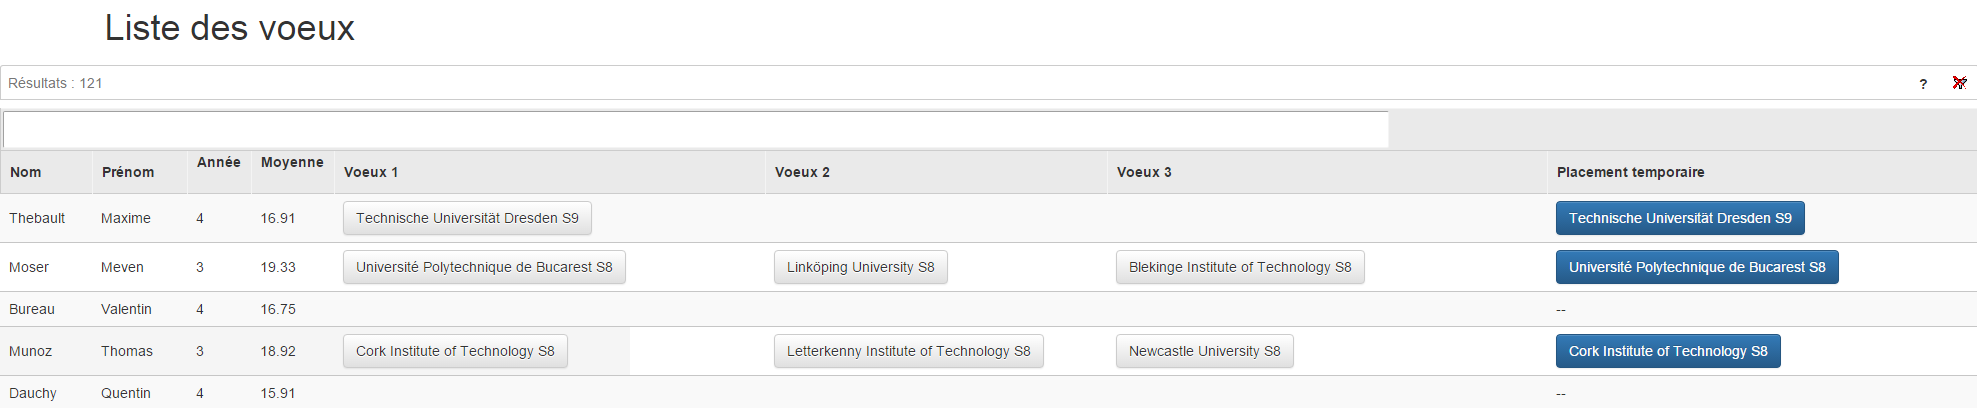
\includegraphics[scale=0.35]{images/lv.png}
	\caption{Liste des vœux}
	\label{lv}
\end{figure}

\section{Gestion d'étudiant}

\subsection{Ajout de vœux}

L'étudiant peut ajouter une université à la liste de ses vœux. Par défaut le nouveau vœux est placé en queue de la liste de vœux de l'élève (cf figure \ref{lus}). Pour faire un vœux, il suffit que l'étudiant choisisse le semestre de départ qui l'intéresse (ou le double diplôme si disponible) puis cliquer sur "ADD" pour que l'ajout soit prit en compte. 
\smallbreak
Si la phase de vœux est verrouillée, l'ajout de nouvelles universités dans la liste de vœux est impossible.

\begin{figure}[H]
	\centering
	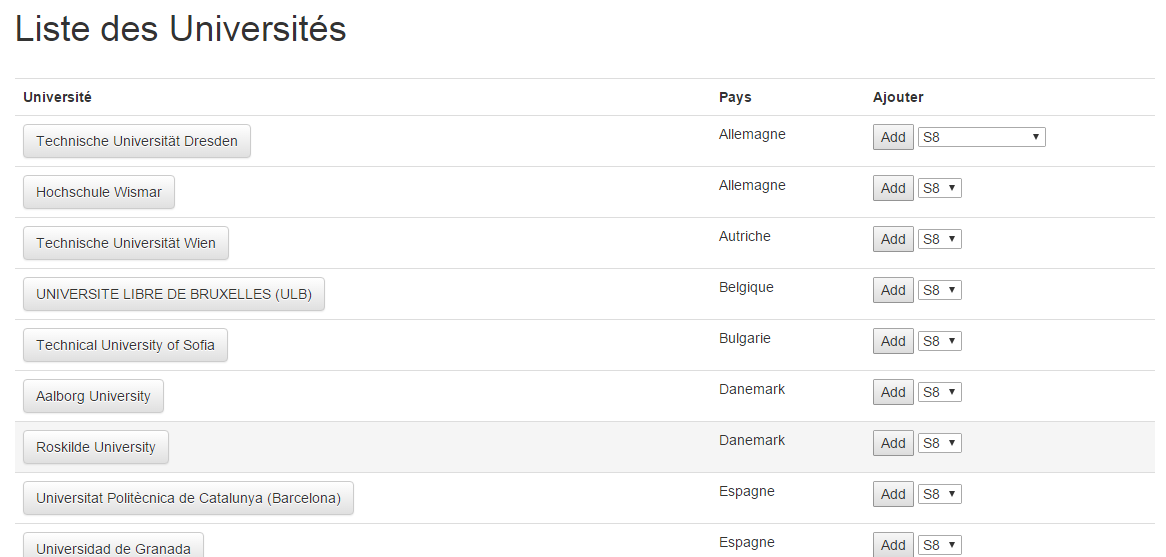
\includegraphics[scale=0.35]{images/LUS.png}
	\caption{Liste des universités}
	\label{lus}
\end{figure}

\subsection{Modification des voeux}

Sur sa page d'accueil, l'étudiant peut voir une liste récapitulative de ses vœux. Lorsque la phase de vœux est active, il peut à loisir modifier l'ordre de ses vœux ainsi que supprimer ces derniers.

\subsection{Ajout learning agreement}

L'élève doit, pour pouvoir faire sa mobilité, soumettre un learning agreement (liste des cours qu'il va suivre à l'étranger). Pour ce faire, un formulaire est à sa disposition. Ce formulaire prend la forme d'une liste de matière auxquelles il attache un nombre de crédits ECTS. Lorsque sa liste est terminée, il la soumet aux administrateurs (cf figure \ref{voeux1}).

\begin{figure}[H]
	\centering
	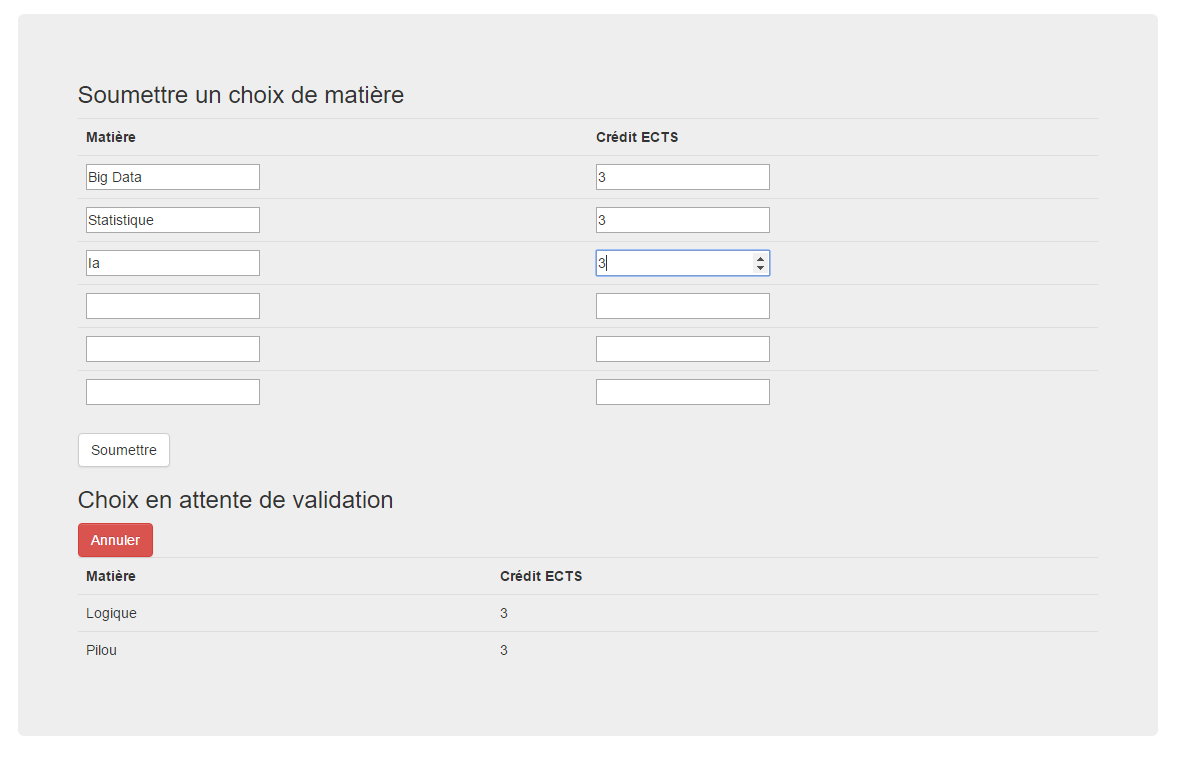
\includegraphics[scale=0.35]{images/voeux1.png}
	\caption{Formulaire de learning agreement}
	\label{voeux1}
\end{figure}

\subsection{Modification du learning agreement}

Même lorsque un learning agreement est validé, il est possible à l'élève d'en soumettre un nouveau si il désire modifier les matières qu'il souhaite étudier. Il lui suffit de remplir alors à nouveau la table et à le soumettre à nouveau (cf figure \ref{voeux2}).

\begin{figure}[H]
	\centering
	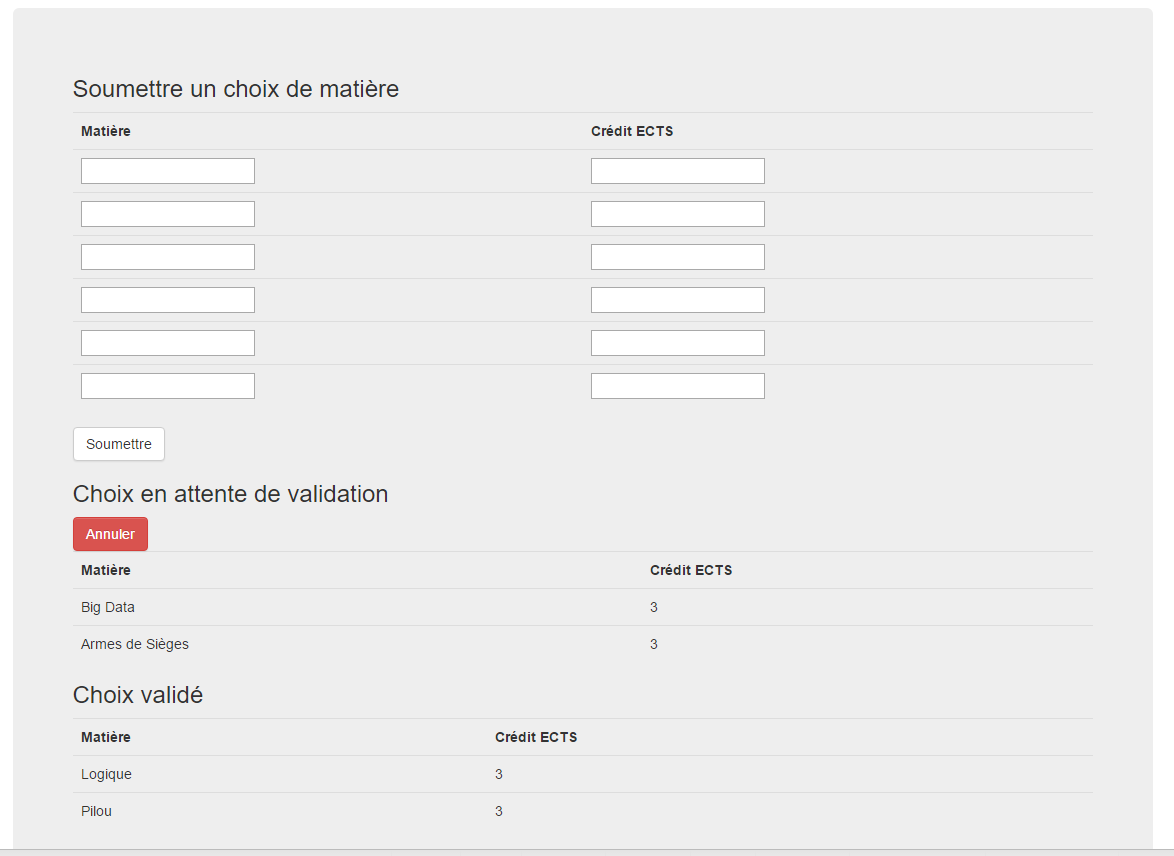
\includegraphics[scale=0.35]{images/voeux2.png}
	\caption{Modification du learning agreement}
	\label{voeux2}
\end{figure}

\subsection{Ajout notes}

Lors de sa mobilité, l'élève va devoir donner à l'INSA les notes qu'il aura obtenu (et qui seront validées par la suite par un document officiel). Pour ce faire, il devra simplement remplir un formulaire contenant la liste de ses matières, et la note obtenue.

\section{Gestion d'administrateur}

\subsection{Ajouter étudiant}

L'administrateur peut ajouter de nouveaux élèves à la base de donnée grâce à son adresse mail INSA. Il peut ajouter les élèves un par un en écrivant l'adresse mail de l'élève suivi de la moyenne de l'élève ou bien effectuer un import CSV au format suivant : sur chaque ligne un mail suivi d'une moyenne (cf figure \ref{ae}).
\smallbreak
Si le mail de l'élève est déjà dans la base de donnée, seul la moyenne est mise à jour.

\begin{figure}[H]
	\centering
	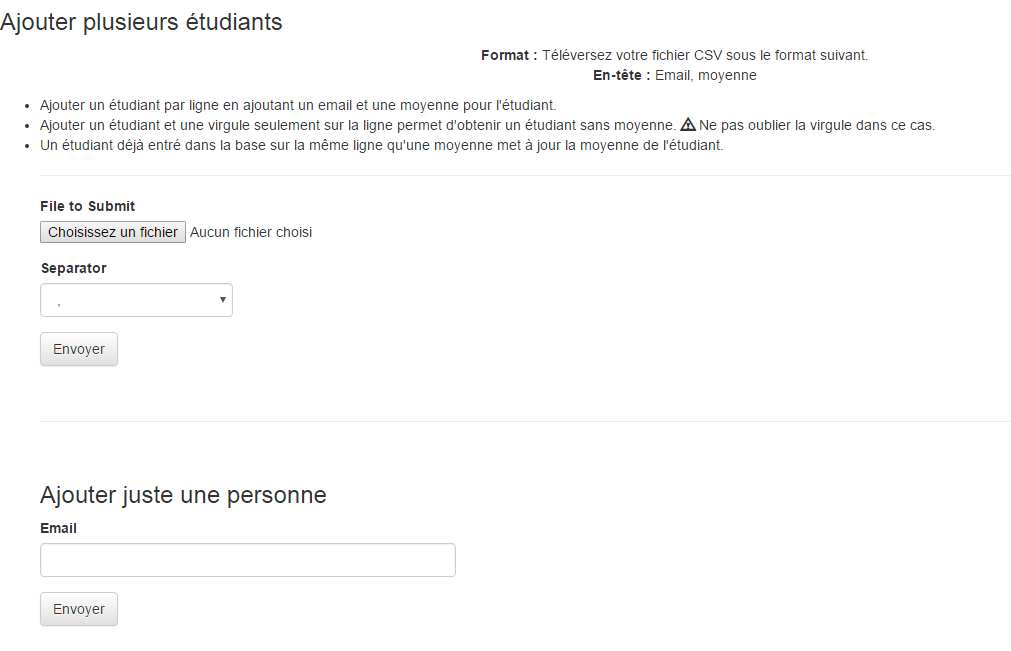
\includegraphics[scale=0.35]{images/ae.png}
	\caption{Page d'ajout des élèves}
	\label{ae}
\end{figure}

\subsection{Inspecter et modifier étudiant} 

L'administrateur peut, en ce rendant sur la page personnelle de l'élève, modifier la moyenne de l'élève sans passer par la page d'ajout d'un élève. De plus, il peut voir si l'élève à été affecté manuellement à une destination et peut écrire et voir un commentaire particulier sur l'élève déposé par n'importe quel administrateur du département (cf figure \ref{psa}.

\begin{figure}[H]
	\centering
	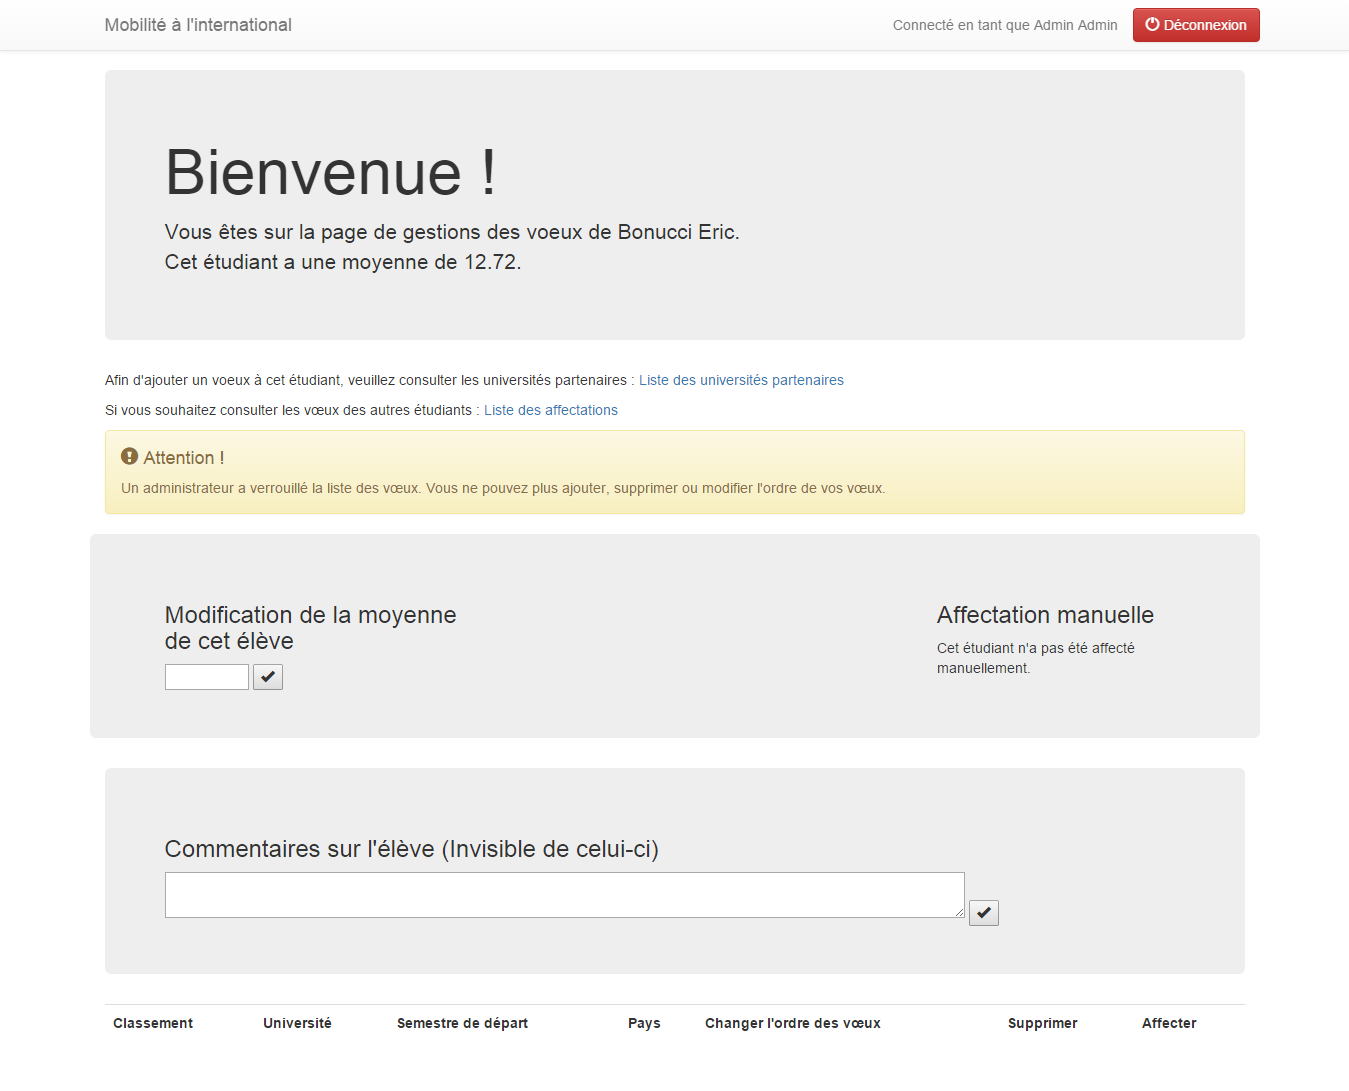
\includegraphics[scale=0.3]{images/psa.png}
	\caption{Page résumé de l'élève}
	\label{psa}
\end{figure}

\subsection{Verrouiller phase de vœux}

Avant de lancer la phase d'affectation des destinations, l'administrateur doit verrouiller la phase de choix afin que les élèves ne puissent plus ajouter ou modifier leurs vœux. Pour ce faire il suffit de cliquer sur un bouton présent sur la page de gestion des affectation (cf figure \ref{ga}).

\subsection{Validation learning agreement}

Lorsqu'un learning agreement est proposé par un élève, il doit être validé par un administrateur. Pour ce faire, l'administrateur n'a qu'à cliquer sur le bouton de validation si le learning agreement convient ou sur le bouton de refus pour refuser (cf figure \ref{lav}).
\smallbreak
Par la suite, lors du refus d'un learning agreement, l'adminstrateur aura la possibilité d'écrire la raison pour laquelle il a refusé.

\begin{figure}[H]
	\centering
	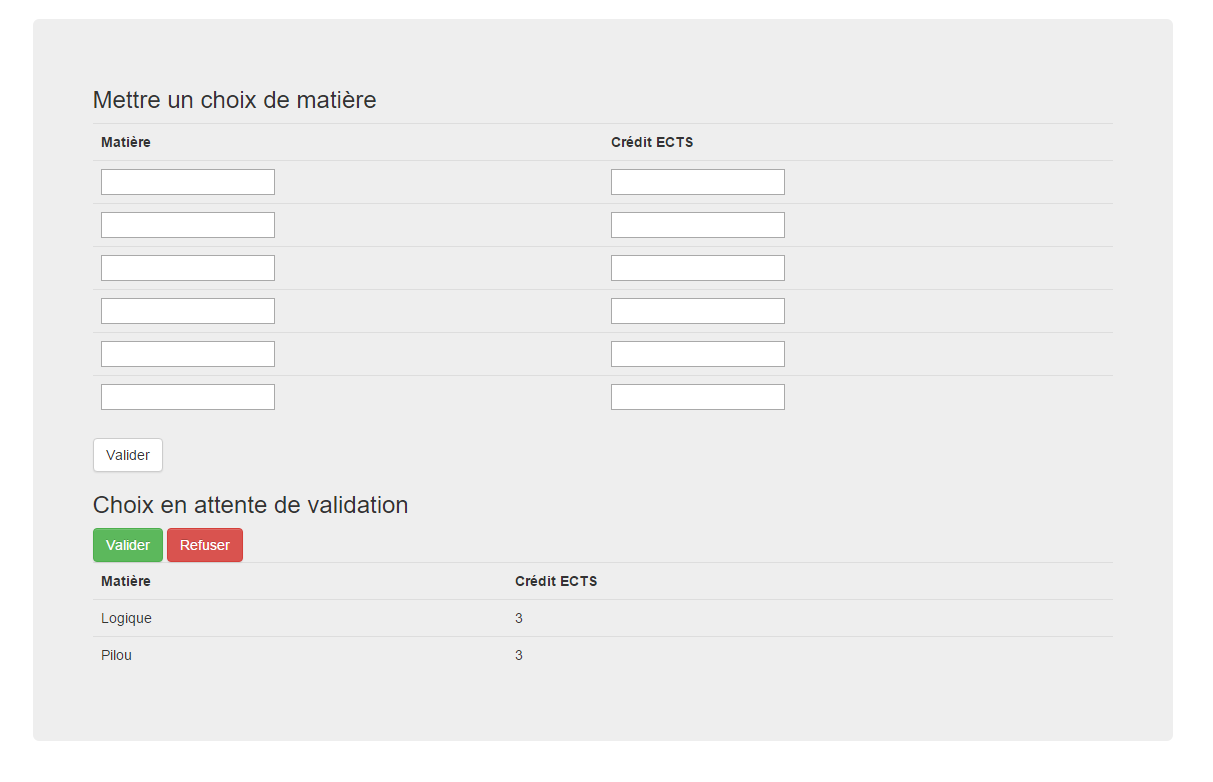
\includegraphics[scale=0.35]{images/lav.png}
	\caption{Validation d'un learning agreement}
	\label{lav}
\end{figure}

